\documentclass[11pt,paper=a4,answers]{exam}
\usepackage{graphicx,lastpage}
\usepackage{upgreek}
\usepackage{censor}
\usepackage{gensymb}
\usepackage{amsmath}
\usepackage{multicol}
\usepackage{enumitem}
\usepackage{tasks}
\usepackage{adjustbox}
\usepackage{pgfplots}
\usepackage{xcolor}
\usepackage{tfrupee}
\setlength{\voffset}{0.25in}
\usepackage{tabularx}
\newcolumntype{Y}{>{\centering\arraybackslash}X}
%==============================================================
% Customise Non-Essential Packages Below
% =============================================================
\usepackage[most]{tcolorbox}
\usepackage{eso-pic}
\usepackage{tikz}
\AddToShipoutPictureBG{%
\begin{tikzpicture}[remember picture,overlay]
\foreach \x in {-8,-4,0,4,8,12,16,20}
\foreach \y in {-8,-4,0,4,8,12,16,20} {
\node[opacity=0.05,rotate=45,anchor=center] at ([xshift=\x cm,yshift=\y cm]current page.center) {%
\begin{minipage}{2cm}
\centering
\includegraphics[width=2cm]{images/logo_black.png}\\
\small preppeo.com
\end{minipage}%
};
}
\end{tikzpicture}%
}
\printanswers

%==============================================================
% Customise Non-Essential Packages Above
% =============================================================
\definecolor{svgray}{rgb}{0.90, 0.90, 0.90}
\graphicspath{{images/}}

\usepackage[normalem]{ulem}
\renewcommand\ULthickness{1pt}   %%---> For changing thickness of underline
\setlength\ULdepth{3.5ex}%\maxdimen ---> For changing depth of underline
\renewcommand{\baselinestretch}{1}
\chead{
\includegraphics[scale=0.1,height=2cm ]{logo.png}
}
\pagestyle{empty}

\pagestyle{headandfoot}
\headrule
\cfoot{W: https://preppeo.com; M: +91-8130711689}

\begin{document}
%==============================================================
% Customise Question paper details below this
% =============================================================
\begin{center}
    \centering
    \renewcommand{\arraystretch}{1.5}
    \begin{tabularx}{\textwidth}{YYY}
    & \normalsize\bf{{\Large{{Quantitative Reasoning}}}} & \\
    By Preppeo & \normalsize\bf{{sat\_lid\_037}} & SAT\\
    \normalsize{{\textbf{{Unit:}} Two-Variable Data}} & \normalsize{{\textbf{{Chapter:}} Scatterplots, trend lines, models}} & \normalsize{{\textbf{{Topic:}} Predictions from Models}} \\
    \end{tabularx}
\end{center}
\par\noindent\rule{\textwidth}{1pt}
% =============================================================
% Customise Question paper details above this
% =============================================================

\begin{questions}
\pointsinrightmargin
\pointsdroppedatright
\marksnotpoints
\pointpoints{mark}{marks}
\pointformat{\boldmath\themarginpoints}
\bracketedpoints

% =============================================================
% Question Begin
% =============================================================

% Question 1
% Category: Exam Level | Difficulty: Medium | Question Type: MCQ
\question
An inspector begins a day of work with a large sample of shirts that need to be checked for defects. The inspector works at a constant rate throughout the morning. What type of model is best to model the number of shirts remaining to be checked for defects at any given time throughout the morning?
\begin{tasks}(1)
    \task A linear model with a positive slope
    \task A linear model with a negative slope
    \task An exponential growth model
    \task An exponential decay model
\end{tasks}

\begin{solution}
\textbf{Conceptual Explanation:} \\
The choice of model depends on two factors: the rate of change and the direction of change. A "constant rate" indicates a linear relationship, while the "number of shirts remaining" indicates the quantity is decreasing over time.

\vspace{30pt}

\textbf{Calculation and Logic:} \\
* The term "constant rate" means that for every equal unit of time, the same number of shirts are checked. This is the definition of a linear function ($y = mx + b$).
* Because the shirts are being checked, the total count of shirts "remaining" must go down as time passes.
* In a linear equation, a decrease over time is represented by a negative slope ($m < 0$).

\vspace{30pt}

Answer: \colorbox{yellow!100}{B}
\end{solution}

\vspace{60pt}

% Question 2
% Category: Practice | Difficulty: Medium | Question Type: MCQ
\question
\begin{center}
\begin{tikzpicture}
\begin{axis}[
    axis lines=middle,
    xmin=0, xmax=10,
    ymin=0, ymax=11,
    xtick={0,2,4,6,8,10},
    ytick={0,2,4,6,8,10},
    grid=major,
    xlabel={$x$},
    ylabel={$y$},
    width=0.5\textwidth
]
\addplot[only marks, mark=*] coordinates {(1,3) (3,5) (5,6) (7,8) (9,10)};
\end{axis}
\end{tikzpicture}
\end{center}
Which equation is the most appropriate linear model for this relationship?
\begin{tasks}(2)
    \task $y = -0.9x - 2.2$
    \task $y = -0.9x + 2.2$
    \task $y = -0.9x$
    \task $y = 0.9x + 2.2$
\end{tasks}

\begin{solution}
\textbf{Conceptual Explanation:} \\
To identify the correct linear model from a scatterplot, we examine the direction of the trend (slope) and the point where the trend would cross the vertical axis (y-intercept).

\vspace{30pt}

\textbf{Calculation and Logic:} \\
* Observe the dots: as $x$ increases, $y$ also increases. This means the slope must be positive ($m > 0$).
* Looking at the choices, only Choice D has a positive slope ($0.9$).
* We can verify the intercept by tracing the trend back to the $y$-axis ($x=0$). The dots align such that the line would cross between 2 and 3, which matches the $+2.2$ intercept in Choice D.

\vspace{30pt}

Answer: \colorbox{yellow!100}{D}
\end{solution}

\vspace{60pt}

% Question 3
% Category: Exam Level | Difficulty: Medium | Question Type: MCQ
\question
An airplane descends from an altitude of 9,500 feet to 5,000 feet at a constant rate of 400 feet per minute. What type of function best models the relationship between the descending airplane's altitude and time?
\begin{tasks}(2)
    \task Decreasing exponential
    \task Decreasing linear
    \task Increasing exponential
    \task Increasing linear
\end{tasks}

\begin{solution}
\textbf{Conceptual Explanation:} \\
Models are determined by how the output changes relative to the input. "Constant rate" always implies linear, and "descends" implies a decrease in altitude.

\vspace{30pt}

\textbf{Calculation and Logic:} \\
* The phrase "constant rate of 400 feet per minute" means that the altitude changes by the exact same amount every minute. This is a linear relationship.
* "Descends" means the altitude is getting smaller as time increases.
* Therefore, the altitude is a decreasing linear function of time.

\vspace{30pt}

Answer: \colorbox{yellow!100}{B}
\end{solution}

\vspace{60pt}

% Question 4
% Category: Exam Level | Difficulty: Hard | Question Type: MCQ
\question
\begin{center}
\begin{tikzpicture}
\begin{axis}[
    xmin=0, xmax=12,
    ymin=700, ymax=830,
    xtick={0,2,4,6,8,10,12},
    ytick={700,720,740,760,780,800,820},
    grid=major,
    xlabel={Time (years)},
    ylabel={Energy (million megawatt-hours)},
    title={Electric Energy Generated by Nuclear Sources},
    width=0.6\textwidth
]
\addplot[only marks, mark=*] coordinates {(1,764) (2,788) (3,781) (4,787) (5,807) (6,806) (7,798) (8,807) (9,789) (10,769)};
\end{axis}
\end{tikzpicture}
\end{center}
Of the following equations, which best models the data in the scatterplot?
\begin{tasks}(2)
    \task $y = 1.674x^2 + 19.76x - 745.73$
    \task $y = -1.674x^2 - 19.76x - 745.73$
    \task $y = 1.674x^2 + 19.76x + 745.73$
    \task $y = -1.674x^2 + 19.76x + 745.73$
\end{tasks}

\begin{solution}
\textbf{Conceptual Explanation:} \\
For a scatterplot that increases and then decreases, a quadratic model ($y = ax^2 + bx + c$) is appropriate. The sign of "a" determines if it opens up or down, and "c" represents the y-intercept.

\vspace{30pt}

\textbf{Calculation and Logic:} \\
* The data points form an "arch" shape, opening downward. This requires the leading coefficient ($a$) to be negative. This eliminates Choices A and C.
* Look at the $y$-values: they are all in the 700--800 range.
* Choice B has a negative intercept ($-745.73$), which would put the graph far below the $x$-axis.
* Choice D has a positive intercept ($+745.73$), which aligns with the observed energy levels.

\vspace{30pt}

Answer: \colorbox{yellow!100}{D}
\end{solution}

\vspace{60pt}

% Question 5
% Category: Practice | Difficulty: Medium | Question Type: MCQ
\question
\begin{center}
\begin{tikzpicture}
\begin{axis}[
    axis lines=middle,
    xmin=0, xmax=6,
    ymin=0, ymax=10,
    xtick={0,1,2,3,4,5,6},
    ytick={0,1,2,3,4,5,6,7,8,9,10},
    grid=major,
    width=0.5\textwidth
]
\addplot[only marks, mark=*] coordinates {(0.5,9.5) (1,8.8) (1.5,7.6) (2,6.5) (2.5,5.8) (3,5) (3.5,3.5) (4,2.8) (4.5,1.6) (5,0.7)};
\end{axis}
\end{tikzpicture}
\end{center}
Which of the following equations is the most appropriate linear model for the data shown in the scatterplot?
\begin{tasks}(2)
    \task $y = -1.9x - 10.1$
    \task $y = -1.9x + 10.1$
    \task $y = 1.9x - 10.1$
    \task $y = 1.9x + 10.1$
\end{tasks}

\begin{solution}
\textbf{Conceptual Explanation:} \\
A linear model is chosen by matching the slope (rate of change) and the intercept (initial value) to the visual trend.

\vspace{30pt}

\textbf{Calculation and Logic:} \\
* The dots slope downward from left to right, indicating a negative slope ($m < 0$). This eliminates C and D.
* The trend line would cross the $y$-axis ($x=0$) near the value 10.
* Choice A has an intercept of $-10.1$, which is incorrect.
* Choice B has an intercept of $+10.1$, which correctly matches the visual data.

\vspace{30pt}

Answer: \colorbox{yellow!100}{B}
\end{solution}

\vspace{60pt}

% Question 6
% Category: Exam Level | Difficulty: Hard | Question Type: MCQ
\question
\begin{center}
\begin{tabular}{|c|c|c|}
\hline
 & Amount invested & Balance increase \\ \hline
Account A & \$500 & 6\% annual interest \\ \hline
Account B & \$1,000 & \$25 per year \\ \hline
\end{tabular}
\end{center}
Two investments were made as shown in the table above. The interest in Account A is compounded once per year. Which of the following is true about the investments?
\begin{tasks}(1)
    \task Account A always earns more money per year than Account B.
    \task Account A always earns less money per year than Account B.
    \task Account A earns more money per year than Account B at first but eventually earns less money per year.
    \task Account A earns less money per year than Account B at first but eventually earns more money per year.
\end{tasks}

\begin{solution}
\textbf{Conceptual Explanation:} \\
This compares linear growth (Account B) with exponential growth (Account A). Linear growth adds a constant amount, while exponential growth adds an increasing amount based on the current total.

\vspace{30pt}

\textbf{Calculation and Logic:} \\
* Account B growth: \$25 every year (constant).
* Account A growth (Year 1): $6\% \text{ of } 500 = \$30$.
* Note: At Year 1, Account A already earns more than B (\$30 $>$ \$25). 
* As the balance in A grows, the 6\% interest will apply to a larger and larger number, making the annual earnings increase over time.
* Since Account A starts higher and grows exponentially, it will always earn more per year than the fixed \$25 in Account B.

\vspace{30pt}

Answer: \colorbox{yellow!100}{A}
\end{solution}

\vspace{60pt}

% Question 7
% Category: Practice | Difficulty: Medium | Question Type: MCQ
\question
\begin{center}
\begin{tikzpicture}
\begin{axis}[
    axis lines=middle,
    xmin=0, xmax=10,
    ymin=0, ymax=10,
    xtick={0,1,2,3,4,5,6,7,8,9,10},
    ytick={0,1,2,3,4,5,6,7,8,9,10},
    grid=major,
    width=0.5\textwidth
]
\addplot[only marks, mark=*] coordinates {(0,10) (1.2,9) (2.4,8) (3.1,5) (4.7,5) (5.3,3) (6.5,3) (7.2,3) (8.7,1) (9.7,2)};
\end{axis}
\end{tikzpicture}
\end{center}
Which of the following equations is the most appropriate linear model for the data shown?
\begin{tasks}(2)
    \task $y = 0.9 + 9.4x$
    \task $y = 0.9 - 9.4x$
    \task $y = 9.4 + 0.9x$
    \task $y = 9.4 - 0.9x$
\end{tasks}

\begin{solution}
\textbf{Conceptual Explanation:} \\
The linear model $y = b + mx$ (or $y = mx + b$) is determined by the $y$-intercept ($b$) and the slope ($m$).

\vspace{30pt}

\textbf{Calculation and Logic:} \\
* Trace the trend to the $y$-axis ($x=0$). The data starts at 10 and stays near high values initially. Choice D's intercept ($9.4$) is the most accurate.
* The dots move down as $x$ increases, so the slope must be negative. This eliminates A and C.
* Choice B has a slope of $-9.4$, which would mean $y$ drops to 0 before $x$ even reaches 1.
* Choice D has a slope of $-0.9$. Testing $x=10$: $y = 9.4 - 0.9(10) = 0.4$. This matches the scatterplot's end point.

\vspace{30pt}

Answer: \colorbox{yellow!100}{D}
\end{solution}

\vspace{60pt}

% Question 8
% Category: Exam Level | Difficulty: Medium | Question Type: MCQ
\question
\begin{center}
\begin{tikzpicture}
\begin{axis}[
    xmin=0, xmax=50,
    ymin=0, ymax=80,
    xtick={0,10,20,30,40,50},
    ytick={0,10,20,30,40,50,60,70,80},
    grid=major,
    xlabel={Total protein (grams)},
    ylabel={Total fat (grams)},
    title={Total Protein and Total Fat for Eight Sandwiches},
    width=0.6\textwidth
]
\addplot[only marks, mark=*] coordinates {(9,16) (14,22) (22,37) (26,44) (28,47) (35,56) (44,70) (49,75)};
\addplot[thick, domain=9:50] {3.5 + 1.48*x};
\end{axis}
\end{tikzpicture}
\end{center}
According to the line of best fit, which of the following is closest to the predicted increase in total fat, in grams, for every increase of 1 gram in total protein?
\begin{tasks}(4)
    \task 2.5
    \task 2.0
    \task 1.5
    \task 1.0
\end{tasks}

\begin{solution}
\textbf{Conceptual Explanation:} \\
The increase in the output ($y$) for every 1-unit increase in the input ($x$) is the definition of the slope of the line of best fit.

\vspace{30pt}

\textbf{Calculation and Logic:} \\
* We need to calculate the slope ($m$) of the line shown in the graph.
* Pick two points on the line: $(10, 18)$ and $(40, 63)$ approximately.
* Calculate the slope: $m = \frac{63 - 18}{40 - 10} = \frac{45}{30} = 1.5$.
* This means for every 1 gram of protein, fat is predicted to increase by 1.5 grams.

\vspace{30pt}

Answer: \colorbox{yellow!100}{C}
\end{solution}

\vspace{60pt}

% Question 9
% Category: Practice | Difficulty: Medium | Question Type: MCQ
\question
Each year, the value of an investment increases by 0.49\% of its value the previous year. Which of the following functions best models how the value of the investment changes over time?
\begin{tasks}(2)
    \task Decreasing exponential
    \task Decreasing linear
    \task Increasing exponential
    \task Increasing linear
\end{tasks}

\begin{solution}
\textbf{Conceptual Explanation:} \\
A "percentage change" of the previous value indicates that the amount of growth changes as the total changes, which is the hallmark of exponential functions.

\vspace{30pt}

\textbf{Calculation and Logic:} \\
* The problem states the value increases by a percentage (0.49\%) of the "value the previous year."
* This means the growth is proportional to the current amount, not a fixed constant. This identifies the function as exponential.
* Since the value is "increasing," the model is an increasing exponential function.

\vspace{30pt}

Answer: \colorbox{yellow!100}{C}
\end{solution}

\vspace{60pt}

% Question 10
% Category: Practice | Difficulty: Medium | Question Type: Numeric Entry
\question
A scatterplot shows the relationship between two variables, $x$ and $y$. The line of best fit is $y = 3.5x + 12$. What is the predicted value of $y$ when $x = 10$?

\begin{solution}
\textbf{Conceptual Explanation:} \\
To make a prediction from a linear model, substitute the given value for the independent variable ($x$) and solve for the dependent variable ($y$).

\vspace{30pt}

\textbf{Calculation and Logic:} \\
* Identify the equation: $y = 3.5x + 12$.
* Substitute $x = 10$ into the equation.
* $y = 3.5(10) + 12$.
* $y = 35 + 12 = 47$.

\vspace{30pt}

Answer: \colorbox{yellow!100}{47}
\end{solution}

% Question 11
% Category: Exam Level | Difficulty: Hard | Question Type: MCQ
\question
A scientist observes that the population of a certain bacteria culture doubles every 4 hours. Which of the following best describes the relationship between the population of the bacteria and the number of hours passed?
\begin{tasks}(1)
    \task Increasing linear
    \task Increasing exponential
    \task Decreasing linear
    \task Decreasing exponential
\end{tasks}

\begin{solution}
\textbf{Conceptual Explanation:} \\
The type of growth is determined by whether the change is a constant amount (linear) or a constant ratio (exponential). Direction is determined by whether the values are becoming larger (increasing) or smaller (decreasing).

\vspace{30pt}

\textbf{Calculation and Logic:} \\
* The term "doubles" indicates that the population is multiplied by 2 at regular intervals. Multiplying by a constant factor is the defining characteristic of an exponential model.
* Since doubling results in a larger number than the previous value, the population is growing.
* Therefore, the relationship is best modeled by an increasing exponential function.

\vspace{30pt}

Answer: \colorbox{yellow!100}{B}
\end{solution}

\vspace{60pt}

% Question 12
% Category: Practice | Difficulty: Medium | Question Type: MCQ
\question
\begin{center}
\begin{tikzpicture}
\begin{axis}[
    axis lines=middle,
    xmin=0, xmax=10,
    ymin=0, ymax=100,
    xtick={0,2,4,6,8,10},
    ytick={0,20,40,60,80,100},
    grid=major,
    xlabel={Weeks},
    ylabel={Balance (\$)},
    width=0.5\textwidth
]
\addplot[only marks, mark=*] coordinates {(1,20) (2,30) (3,40) (4,50) (5,60) (6,70)};
\addplot[thick, domain=0:8] {10 + 10*x};
\end{axis}
\end{tikzpicture}
\end{center}
The scatterplot and line of best fit show the balance of a savings account over several weeks. What is the predicted balance after 9 weeks?
\begin{tasks}(4)
    \task \$80
    \task \$90
    \task \$100
    \task \$110
\end{tasks}

\begin{solution}
\textbf{Conceptual Explanation:} \\
Predictions for values outside the plotted data points (extrapolation) are made by extending the line of best fit or using its equation.

\vspace{30pt}

\textbf{Calculation and Logic:} \\
* Identify the slope of the line: The points follow a pattern of increasing by $10 for every 1 week.
* Identify the intercept: The line starts at $10 when Weeks = 0.
* Use the linear model: $y = 10x + 10$.
* Substitute $x = 9$: $y = 10(9) + 10 = 90 + 10 = 100$.

\vspace{30pt}

Answer: \colorbox{yellow!100}{C}
\end{solution}

\vspace{60pt}

% Question 13
% Category: Exam Level | Difficulty: Hard | Question Type: MCQ
\question
A linear model is used to predict the value, $v$, of a piece of equipment $t$ years after it was purchased. The equation is $v = 15,000 - 1,200t$. Which of the following is the best interpretation of the value 1,200 in this context?
\begin{tasks}(1)
    \task The total value of the equipment after 1 year.
    \task The predicted decrease in the value of the equipment each year.
    \task The initial cost of the equipment.
    \task The number of years until the equipment has no value.
\end{tasks}

\begin{solution}
\textbf{Conceptual Explanation:} \\
In a linear equation of the form $y = mx + b$ or $y = b - mx$, the coefficient of the variable (the slope $m$) represents the rate of change per unit of time.

\vspace{30pt}

\textbf{Calculation and Logic:} \\
* In the equation $v = 15,000 - 1,200t$, 1,200 is the slope.
* Because it is being subtracted, it represents a decrease in the value $v$.
* The variable $t$ is measured in years, so 1,200 is the rate of decrease per year.

\vspace{30pt}

Answer: \colorbox{yellow!100}{B}
\end{solution}

\vspace{60pt}

% Question 14
% Category: Practice | Difficulty: Medium | Question Type: Numeric Entry
\question
\begin{center}
\begin{tikzpicture}
\begin{axis}[
    axis lines=middle,
    xmin=0, xmax=5,
    ymin=0, ymax=25,
    xtick={0,1,2,3,4,5},
    ytick={0,5,10,15,20,25},
    grid=major,
    width=0.5\textwidth
]
\addplot[thick, samples=50, domain=0:5] {x^2};
\end{axis}
\end{tikzpicture}
\end{center}
The graph shows a model for the area of a square, $y$, given its side length, $x$. Based on the model, what is the area when the side length is 4.5?

\begin{solution}
\textbf{Conceptual Explanation:} \\
For quadratic models representing area, the relationship is $y = x^2$. To find a specific value, square the input.

\vspace{30pt}

\textbf{Calculation and Logic:} \\
* The input value is $x = 4.5$.
* Apply the squaring model: $4.5 \times 4.5$.
* Calculation: $4.5 \times 4.5 = 20.25$.

\vspace{30pt}

Answer: \colorbox{yellow!100}{20.25}
\end{solution}

\vspace{60pt}

% Question 15
% Category: Exam Level | Difficulty: Hard | Question Type: MCQ
\question
\begin{center}
\begin{tikzpicture}
\begin{axis}[
    axis lines=middle,
    xmin=0, xmax=10,
    ymin=0, ymax=10,
    xtick={0,2,4,6,8,10},
    ytick={0,2,4,6,8,10},
    grid=major,
    width=0.5\textwidth
]
\addplot[only marks, mark=*] coordinates {(1,9) (2,7) (3,6) (4,4) (5,3.5) (6,2) (8,1)};
\addplot[thick, domain=0:10] {10 - 1.15*x};
\end{axis}
\end{tikzpicture}
\end{center}
For the scatterplot shown, which of the following is the best estimate for the residual of the data point at $x = 3$?
\begin{tasks}(4)
    \task -0.5
    \task 0.5
    \task 1.5
    \task 6.5
\end{tasks}

\begin{solution}
\textbf{Conceptual Explanation:} \\
A residual is the vertical distance between an actual data point ($y_{actual}$) and the value predicted by the line of best fit ($y_{predicted}$). 
\[ \text{Residual} = y_{actual} - y_{predicted} \]

\vspace{30pt}

\textbf{Calculation and Logic:} \\
* Identify $y_{actual}$: At $x = 3$, the data point is at $y = 6$.
* Identify $y_{predicted}$: Looking at the line at $x = 3$, it is slightly above 6.5 (approximately 6.55).
* Calculate the difference: $6 - 6.55 \approx -0.55$.
* A negative residual indicates the actual point is below the line. Choice A is the closest estimate.

\vspace{30pt}

Answer: \colorbox{yellow!100}{A}
\end{solution}

\vspace{60pt}

% Question 16
% Category: Concept | Difficulty: Medium | Question Type: MCQ
\question
Which of the following scatterplots would be best modeled by an equation of the form $y = a(b)^x$ where $a > 0$ and $0 < b < 1$?
\begin{tasks}(1)
    \task Points that form a straight line sloping upward.
    \task Points that form a straight line sloping downward.
    \task Points that form a curve getting steeper as $x$ increases.
    \task Points that form a curve getting flatter as $x$ increases.
\end{tasks}

\begin{solution}
\textbf{Conceptual Explanation:} \\
The equation $y = a(b)^x$ is an exponential model. If the base $b$ is between 0 and 1, the model represents exponential decay.

\vspace{30pt}

\textbf{Calculation and Logic:} \\
* Exponential decay curves always decrease as $x$ increases.
* As $x$ gets larger, the $y$-values decrease but at a slower and slower rate, causing the curve to "flatten out" toward the $x$-axis.
* Linear models (straight lines) do not match this functional form.

\vspace{30pt}

Answer: \colorbox{yellow!100}{D}
\end{solution}

\vspace{60pt}

% Question 17
% Category: Practice | Difficulty: Medium | Question Type: MCQ
\question
A line of best fit is given by $\hat{y} = -2.5x + 50$. For which of the following values of $x$ is the predicted value of $y$ equal to 10?
\begin{tasks}(4)
    \task 10
    \task 16
    \task 20
    \task 24
\end{tasks}

\begin{solution}
\textbf{Calculation and Logic:} \\
* Set the predicted value $\hat{y}$ to 10.
* $10 = -2.5x + 50$.
* Subtract 50 from both sides: $-40 = -2.5x$.
* Divide by $-2.5$: $x = \frac{-40}{-2.5} = 16$.

\vspace{30pt}

Answer: \colorbox{yellow!100}{B}
\end{solution}

\vspace{60pt}

% Question 18
% Category: Exam Level | Difficulty: Hard | Question Type: MCQ
\question
\begin{center}
\begin{tikzpicture}
\begin{axis}[
    axis lines=middle,
    xmin=0, xmax=10,
    ymin=0, ymax=10,
    xtick={0,2,4,6,8,10},
    ytick={0,2,4,6,8,10},
    grid=major,
    width=0.45\textwidth
]
\addplot[only marks, mark=*] coordinates {(1,2.5) (2,3.5) (4,5.5) (6,7.5) (8,9.5)};
\addplot[thick, domain=0:8] {1.5 + 1.0*x};
\end{axis}
\end{tikzpicture}
\end{center}
What is the slope of the line of best fit shown?
\begin{tasks}(4)
    \task 0.5
    \task 1.0
    \task 1.5
    \task 2.5
\end{tasks}

\begin{solution}
\textbf{Conceptual Explanation:} \\
The slope ($m$) represents the "rise over run"—the amount the line goes up vertically for every 1 unit it moves horizontally.

\vspace{30pt}

\textbf{Calculation and Logic:} \\
* Select two points on the line: $(0, 1.5)$ and $(4, 5.5)$.
* Apply slope formula: $m = \frac{5.5 - 1.5}{4 - 0} = \frac{4}{4} = 1.0$.
* This indicates that for every 1 unit increase in $x$, $y$ increases by 1 unit.

\vspace{30pt}

Answer: \colorbox{yellow!100}{B}
\end{solution}

\vspace{60pt}

% Question 19
% Category: Practice | Difficulty: Easy | Question Type: Numeric Entry
\question
A model predicts the total cost $C$ of an item including 8% tax as $C = 1.08p$, where $p$ is the original price. If the original price is $50, what is the predicted total cost?

\begin{solution}
\textbf{Calculation and Logic:} \\
* Identify the model: $C = 1.08p$.
* Substitute $p = 50$: $C = 1.08(50)$.
* Multiplication: $1.08 \times 50 = 54$.

\vspace{30pt}

Answer: \colorbox{yellow!100}{54}
\end{solution}

\vspace{60pt}

% Question 20
% Category: Exam Level | Difficulty: Hard | Question Type: MCQ
\question
Which of the following best describes the difference between a linear model and an exponential model?
\begin{tasks}(1)
    \task Linear models always increase, while exponential models always decrease.
    \task Linear models have a constant rate of change, while exponential models have a constant ratio of change.
    \task Linear models are for small data sets, while exponential models are for large data sets.
    \task Linear models must pass through the origin (0,0).
\end{tasks}

\begin{solution}
\textbf{Conceptual Explanation:} \\
The fundamental difference lies in how the "next" value is calculated.

\vspace{30pt}

\textbf{Calculation and Logic:} \\
* In a linear model ($y = mx + b$), you add the same amount ($m$) every time $x$ increases by 1. This is a constant rate.
* In an exponential model ($y = ab^x$), you multiply by the same factor ($b$) every time $x$ increases by 1. This is a constant ratio or percentage.

\vspace{30pt}

Answer: \colorbox{yellow!100}{B}
\end{solution}

% Question 21
% Category: Exam Level | Difficulty: Hard | Question Type: MCQ
\question
A scientist uses the model $P = 100(1.04)^t$ to predict the population of a town $t$ years after a census was taken. Which of the following is the best interpretation of the value 1.04 in this context?
\begin{tasks}(1)
    \task The population increases by 4 people each year.
    \task The population increases by 104 people each year.
    \task The population increases by 4\% each year.
    \task The population increases by 104\% each year.
\end{tasks}

\begin{solution}
\textbf{Conceptual Explanation:} \\
In an exponential growth model $y = a(b)^x$, the base $b$ represents the growth factor. If $b > 1$, the growth rate $r$ can be found using the relationship $b = 1 + r$.

\vspace{30pt}

\textbf{Calculation and Logic:} \\
* Identify the base $b$ in the equation $P = 100(1.04)^t$, which is 1.04.
* Set up the growth rate equation: $1.04 = 1 + r$.
* Solve for $r$: $r = 0.04$.
* Convert the decimal to a percentage: $0.04 \times 100 = 4\%$.
* This means the population grows by 4\% of its current value every year.

\vspace{30pt}

Answer: \colorbox{yellow!100}{C}
\end{solution}

\vspace{60pt}

% Question 22
% Category: Practice | Difficulty: Medium | Question Type: Numeric Entry
\question
A line of best fit for a scatterplot is $y = -0.5x + 120$. What is the predicted value of $y$ when $x = 80$?

\begin{solution}
\textbf{Conceptual Explanation:} \\
To find a predicted value, we perform a substitution into the mathematical model provided.

\vspace{30pt}

\textbf{Calculation and Logic:} \\
* Use the equation: $y = -0.5x + 120$.
* Substitute $x = 80$ into the expression.
* $y = -0.5(80) + 120$.
* Calculate the product: $-0.5 \times 80 = -40$.
* Sum the values: $-40 + 120 = 80$.

\vspace{30pt}

Answer: \colorbox{yellow!100}{80}
\end{solution}

\vspace{60pt}

% Question 23
% Category: Exam Level | Difficulty: Medium | Question Type: MCQ
\question
\begin{center}
\begin{tikzpicture}
\begin{axis}[
    axis lines=middle,
    xmin=0, xmax=10,
    ymin=0, ymax=10,
    xtick={0,2,4,6,8,10},
    ytick={0,2,4,6,8,10},
    grid=major,
    width=0.45\textwidth
]
\addplot[only marks, mark=*] coordinates {(1,8) (2,7.5) (3,6) (5,5) (7,4) (9,2)};
\addplot[thick, domain=0:10] {9 - 0.75*x};
\end{axis}
\end{tikzpicture}
\end{center}
The scatterplot shows the relationship between two variables, and a line of best fit is shown. Which of the following is the best estimate for the $y$-intercept of the line?
\begin{tasks}(4)
    \task 0
    \task 7.5
    \task 9.0
    \task 10.0
\end{tasks}

\begin{solution}
\textbf{Conceptual Explanation:} \\
The $y$-intercept is the point where the line of best fit intersects the vertical axis ($x = 0$).

\vspace{30pt}

\textbf{Calculation and Logic:} \\
* Locate the vertical $y$-axis on the graph.
* Follow the line of best fit back to where it touches this axis.
* The line crosses the axis at the grid mark for 9.
* Therefore, the initial value (or $y$-intercept) of this model is 9.0.

\vspace{30pt}

Answer: \colorbox{yellow!100}{C}
\end{solution}

\vspace{60pt}

% Question 24
% Category: Practice | Difficulty: Hard | Question Type: MCQ
\question
The volume of a gas decreases at a constant rate as the pressure increases. If the volume is 100 liters at 2 atmospheres and 80 liters at 4 atmospheres, what is the predicted volume at 10 atmospheres?
\begin{tasks}(4)
    \task 20 liters
    \task 40 liters
    \task 50 liters
    \task 60 liters
\end{tasks}

\begin{solution}
\textbf{Conceptual Explanation:} \\
"Constant rate" indicates a linear model. We must find the rate of change (slope) to predict future values.

\vspace{30pt}

\textbf{Calculation and Logic:} \\
* Identify the two points: $(2, 100)$ and $(4, 80)$.
* Calculate the slope ($m$): $m = \frac{80 - 100}{4 - 2} = \frac{-20}{2} = -10$ liters per atmosphere.
* Determine the model: $y = -10x + b$. Use $(2, 100)$ to find $b$: $100 = -10(2) + b \Rightarrow b = 120$.
* Predict for $x = 10$: $y = -10(10) + 120 = -100 + 120 = 20$.

\vspace{30pt}

Answer: \colorbox{yellow!100}{A}
\end{solution}

\vspace{60pt}

% Question 25
% Category: Exam Level | Difficulty: Medium | Question Type: MCQ
\question
A manager uses the model $\hat{y} = 15x + 200$ to predict total sales, where $x$ is the number of customers. If the actual sales for 10 customers was \$340, what is the residual for this data point?
\begin{tasks}(4)
    \task -\$10
    \task \$10
    \task -\$350
    \task \$350
\end{tasks}

\begin{solution}
\textbf{Conceptual Explanation:} \\
A residual is the difference between the actual observed value and the value predicted by the model. 
\[ \text{Residual} = \text{Actual} - \text{Predicted} \]

\vspace{30pt}

\textbf{Calculation and Logic:} \\
* Calculate the predicted value ($\hat{y}$) for $x = 10$: $\hat{y} = 15(10) + 200 = 150 + 200 = 350$.
* Identify the actual value: $y = 340$.
* Calculate the residual: $340 - 350 = -10$.
* The negative sign indicates the actual sales were \$10 lower than the model predicted.

\vspace{30pt}

Answer: \colorbox{yellow!100}{A}
\end{solution}

\vspace{60pt}

% Question 26
% Category: Practice | Difficulty: Medium | Question Type: MCQ
\question
Which of the following describes the behavior of an exponential decay model?
\begin{tasks}(1)
    \task The values decrease by a constant amount each period.
    \task The values increase by a constant percentage each period.
    \task The values decrease by a constant percentage each period.
    \task The values remain constant over time.
\end{tasks}

\begin{solution}
\textbf{Conceptual Explanation:} \\
Exponential models are defined by a constant ratio or percentage change. Decay specifically refers to a decrease in value.

\vspace{30pt}

\textbf{Calculation and Logic:} \\
* Choice A describes a linear model (constant amount).
* Choice B describes exponential growth (increasing percentage).
* Choice C describes exponential decay (decreasing percentage). This is the correct definition.

\vspace{30pt}

Answer: \colorbox{yellow!100}{C}
\end{solution}

\vspace{60pt}

% Question 27
% Category: Exam Level | Difficulty: Hard | Question Type: Numeric Entry
\question
A scientist models the height of a projectile with $h = -5t^2 + 20t + 2$, where $h$ is height in meters and $t$ is time in seconds. What is the predicted height of the projectile 3 seconds after it is launched?

\begin{solution}
\textbf{Calculation and Logic:} \\
* Substitute $t = 3$ into the quadratic equation.
* $h = -5(3)^2 + 20(3) + 2$.
* Calculate the exponent: $3^2 = 9$.
* Multiply: $-5 \times 9 = -45$ and $20 \times 3 = 60$.
* Combine the terms: $-45 + 60 + 2$.
* Final result: $15 + 2 = 17$.

\vspace{30pt}

Answer: \colorbox{yellow!100}{17}
\end{solution}

\vspace{60pt}

% Question 28
% Category: Practice | Difficulty: Medium | Question Type: MCQ
\question
If a line of best fit has a slope of 0.8, what is the predicted change in $y$ if $x$ increases by 5 units?
\begin{tasks}(4)
    \task 0.8
    \task 4.0
    \task 5.0
    \task 5.8
\end{tasks}

\begin{solution}
\textbf{Conceptual Explanation:} \\
The slope represents the change in $y$ for a single-unit change in $x$. For larger changes in $x$, we multiply the change by the slope.

\vspace{30pt}

\textbf{Calculation and Logic:} \\
* Identify the slope: $m = 0.8$.
* Identify the change in $x$: $\Delta x = 5$.
* Use the formula for change: $\Delta y = m \times \Delta x$.
* Calculate: $0.8 \times 5 = 4.0$.

\vspace{30pt}

Answer: \colorbox{yellow!100}{B}
\end{solution}

\vspace{60pt}

% Question 29
% Category: Exam Level | Difficulty: Hard | Question Type: MCQ
\question
\begin{center}
\begin{tikzpicture}
\begin{axis}[
    axis lines=middle,
    xmin=0, xmax=5,
    ymin=0, ymax=10,
    xtick={0,1,2,3,4,5},
    ytick={0,2,4,6,8,10},
    grid=major,
    width=0.45\textwidth
]
\addplot[thick, domain=0:4] {8 * (0.5^x)};
\end{axis}
\end{tikzpicture}
\end{center}
Based on the exponential model shown, which of the following is true about the relationship between $x$ and $y$?
\begin{tasks}(1)
    \task As $x$ increases by 1, $y$ decreases by 0.5.
    \task As $x$ increases by 1, $y$ decreases by 50\%.
    \task As $x$ increases by 1, $y$ increases by 50\%.
    \task As $x$ increases by 1, $y$ stays the same.
\end{tasks}

\begin{solution}
\textbf{Conceptual Explanation:} \\
In the model $y = a(b)^x$, the base $b$ represents the ratio of any $y$-value to the previous $y$-value.

\vspace{30pt}

\textbf{Calculation and Logic:} \\
* Observe the graph: at $x=0, y=8$; at $x=1, y=4$; at $x=2, y=2$.
* Each time $x$ increases by 1, the $y$-value is cut in half ($8 \rightarrow 4 \rightarrow 2$).
* Cutting a value in half is equivalent to a 50\% decrease.
* Choice A is incorrect because it implies a constant amount (linear), but the decrease changes (from $-4$ to $-2$).

\vspace{30pt}

Answer: \colorbox{yellow!100}{B}
\end{solution}

\vspace{60pt}

% Question 30
% Category: Practice | Difficulty: Easy | Question Type: MCQ
\question
A scatterplot shows a perfect positive correlation ($r = 1$). If the line of best fit passes through $(2, 5)$ and has a slope of 3, what is the $y$-intercept?
\begin{tasks}(4)
    \task -1
    \task 1
    \task 2
    \task 3
\end{tasks}

\begin{solution}
\textbf{Calculation and Logic:} \\
* Use the slope-intercept form: $y = mx + b$.
* Substitute the known slope ($m=3$) and the point $(2, 5)$.
* $5 = 3(2) + b$.
* $5 = 6 + b$.
* $b = 5 - 6 = -1$.

\vspace{30pt}

Answer: \colorbox{yellow!100}{A}
\end{solution}

\vspace{60pt}

% Question 31
% Category: Exam Level | Difficulty: Hard | Question Type: MCQ
\question
A model predicts that the value of a car depreciates according to the equation $y = 25000(0.85)^t$. What is the predicted value after 2 years?
\begin{tasks}(4)
    \task \$18,062.50
    \task \$21,250.00
    \task \$15,354.25
    \task \$12,500.00
\end{tasks}

\begin{solution}
\textbf{Calculation and Logic:} \\
* Identify the model: $y = 25000(0.85)^t$.
* Substitute $t = 2$: $y = 25000(0.85)^2$.
* Calculate the exponent: $0.85 \times 0.85 = 0.7225$.
* Multiply by the initial value: $25000 \times 0.7225 = 18062.5$.

\vspace{30pt}

Answer: \colorbox{yellow!100}{A}
\end{solution}

\vspace{60pt}

% Question 32
% Category: Concept | Difficulty: Medium | Question Type: MCQ
\question
What does a residual of 0 for a specific data point imply?
\begin{tasks}(1)
    \task The data point is an outlier.
    \task The line of best fit perfectly predicts the value of that point.
    \task The correlation of the entire data set is 1.
    \task The slope of the line is 0.
\end{tasks}

\begin{solution}
\textbf{Logic:} \\
* Residual = Actual $-$ Predicted.
* If the residual is 0, then Actual = Predicted.
* This means the data point lies exactly on the line of best fit.

\vspace{30pt}

Answer: \colorbox{yellow!100}{B}
\end{solution}

\vspace{60pt}

% Question 33
% Category: Practice | Difficulty: Medium | Question Type: Numeric Entry
\question
The line of best fit for a set of data is $y = 2x + 5$. What is the predicted $x$-value when $y = 25$?

\begin{solution}
\textbf{Calculation:} \\
* Set $y = 25$: $25 = 2x + 5$.
* Subtract 5: $20 = 2x$.
* Divide by 2: $x = 10$.

\vspace{30pt}

Answer: \colorbox{yellow!100}{10}
\end{solution}

\vspace{60pt}

% Question 34
% Category: Exam Level | Difficulty: Hard | Question Type: MCQ
\question
Which of the following would be the best model for a data set where the $y$-values are 10, 20, 40, 80, 160 for $x$-values 1, 2, 3, 4, 5?
\begin{tasks}(2)
    \task $y = 10x$
    \task $y = 5(2)^x$
    \task $y = 10x^2$
    \task $y = 2x + 8$
\end{tasks}

\begin{solution}
\textbf{Logic:} \\
* Check the pattern: $10 \times 2 = 20, 20 \times 2 = 40, 40 \times 2 = 80$.
* This is a doubling pattern (constant ratio), which is exponential.
* Test Choice B: $5(2)^1 = 10$; $5(2)^2 = 20$; $5(2)^3 = 40$. It matches perfectly.

\vspace{30pt}

Answer: \colorbox{yellow!100}{B}
\end{solution}

\vspace{60pt}

% Question 35
% Category: Practice | Difficulty: Medium | Question Type: MCQ
\question
A scatterplot has a negative correlation. What does this mean for the line of best fit?
\begin{tasks}(1)
    \task The line will have a positive slope.
    \task The line will have a negative slope.
    \task The line will be horizontal.
    \task The line will be vertical.
\end{tasks}

\begin{solution}
\textbf{Logic:} \\
* Negative correlation means as $x$ increases, $y$ decreases.
* A decreasing trend is represented by a line with a negative slope.

\vspace{30pt}

Answer: \colorbox{yellow!100}{B}
\end{solution}

% Question 36
% Category: Practice | Difficulty: Medium | Question Type: MCQ
\question
A scatterplot of $(x, y)$ data is shown, and the line of best fit is $y = 0.8x + 4.2$. Which of the following is the predicted $y$-value when $x = 5$?
\begin{tasks}(4)
    \task 4.0
    \task 8.2
    \task 10.2
    \task 21.0
\end{tasks}

\begin{solution}
\textbf{Conceptual Explanation:} \\
In SAT math, making a "prediction" using a linear model requires evaluating the function at a specific input value. The line of best fit represents the "expected" value of the dependent variable for any given independent variable.

\vspace{30pt}

\textbf{Calculation and Logic:} \\
* Use the provided model: $y = 0.8x + 4.2$.
* Substitute $x = 5$ into the equation.
* Multiply the coefficients: $0.8 \times 5 = 4.0$.
* Add the $y$-intercept: $4.0 + 4.2 = 8.2$.

\vspace{30pt}

Answer: \colorbox{yellow!100}{B}
\end{solution}

\vspace{60pt}

% Question 37
% Category: Exam Level | Difficulty: Hard | Question Type: MCQ
\question
The equation $y = 12.5(1.08)^x$ models the population of a certain species in a park $x$ years after 2010. Which of the following is the best interpretation of the number 12.5 in this context?
\begin{tasks}(1)
    \task The population increases by 12.5\% each year.
    \task The predicted population of the species in 2010 was 12.5.
    \task The predicted population of the species in 2011 was 12.5.
    \task The species will become extinct in 12.5 years.
\end{tasks}

\begin{solution}
\textbf{Conceptual Explanation:} \\
In the exponential form $y = a(b)^x$, the value of $a$ represents the initial value, or the value of $y$ when $x = 0$.

\vspace{30pt}

\textbf{Calculation and Logic:} \\
* The variable $x$ is defined as years after 2010.
* For the year 2010, $x = 0$.
* Substitute $x = 0$ into the model: $y = 12.5(1.08)^0$.
* Since any non-zero number to the power of 0 is 1, $y = 12.5(1) = 12.5$.
* This confirms that 12.5 is the predicted population at the starting point (2010).

\vspace{30pt}

Answer: \colorbox{yellow!100}{B}
\end{solution}

\vspace{60pt}

% Question 38
% Category: Practice | Difficulty: Medium | Question Type: MCQ
\question
\begin{center}
\begin{tikzpicture}
\begin{axis}[
    axis lines=middle,
    xmin=0, xmax=10,
    ymin=0, ymax=10,
    xtick={0,2,4,6,8,10},
    ytick={0,2,4,6,8,10},
    grid=major,
    width=0.45\textwidth
]
\addplot[only marks, mark=*] coordinates {(2,5) (4,7) (6,8) (8,9)};
\addplot[thick, domain=0:10] {4 + 0.65*x};
\end{axis}
\end{tikzpicture}
\end{center}
A line of best fit for the data is shown. For which of the following $x$-values is the actual $y$-value greater than the predicted $y$-value?
\begin{tasks}(4)
    \task $x = 2$
    \task $x = 4$
    \task $x = 6$
    \task $x = 8$
\end{tasks}

\begin{solution}
\textbf{Conceptual Explanation:} \\
The line of best fit represents the predicted values. If a data point (dot) is located above the line, the actual value is greater than the predicted value. This results in a positive residual.

\vspace{30pt}

\textbf{Calculation and Logic:} \\
* Scan the scatterplot at each provided $x$-value.
* At $x = 2$, the dot is above the line.
* At $x = 4$, the dot is on the line.
* At $x = 6$ and $x = 8$, the dots are below the line.
* Therefore, the actual value is greater than the predicted value only at $x = 2$.

\vspace{30pt}

Answer: \colorbox{yellow!100}{A}
\end{solution}

\vspace{60pt}

% Question 39
% Category: Exam Level | Difficulty: Hard | Question Type: Numeric Entry
\question
A scientist uses the model $f(t) = 100 - 4.9t^2$ to predict the height of an object, in meters, $t$ seconds after it is dropped from a tower. What is the predicted height of the object, in meters, 4 seconds after it is dropped?

\begin{solution}
\textbf{Conceptual Explanation:} \\
This is a quadratic decay model representing free-fall. To find the height at a specific time, perform the operations in the order of PEMDAS (Exponents, then Multiplication, then Subtraction).

\vspace{30pt}

\textbf{Calculation and Logic:} \\
* Identify the model: $f(4) = 100 - 4.9(4)^2$.
* Calculate the square of the time: $4^2 = 16$.
* Multiply the coefficient by the square: $4.9 \times 16 = 78.4$.
* Subtract the result from the initial height: $100 - 78.4 = 21.6$.

\vspace{30pt}

Answer: \colorbox{yellow!100}{21.6}
\end{solution}

\vspace{60pt}

% Question 40
% Category: Practice | Difficulty: Medium | Question Type: MCQ
\question
If the equation of the line of best fit for a scatterplot is $y = -2x + 15$, which of the following is true?
\begin{tasks}(1)
    \task As $x$ increases by 1, $y$ increases by 2.
    \task As $x$ increases by 1, $y$ decreases by 2.
    \task As $x$ increases by 1, $y$ increases by 15.
    \task As $x$ increases by 1, $y$ decreases by 15.
\end{tasks}

\begin{solution}
\textbf{Conceptual Explanation:} \\
The slope ($m$) in $y = mx + b$ represents the constant rate of change. It describes the vertical change for every 1-unit horizontal change.

\vspace{30pt}

\textbf{Calculation and Logic:} \\
* Identify the slope from the equation: $m = -2$.
* A negative slope indicates that the dependent variable ($y$) decreases as the independent variable ($x$) increases.
* The value 2 tells us the magnitude of that decrease.
* Thus, for every 1-unit increase in $x$, $y$ is predicted to decrease by 2 units.

\vspace{30pt}

Answer: \colorbox{yellow!100}{B}
\end{solution}

\vspace{60pt}

% Question 41
% Category: Exam Level | Difficulty: Hard | Question Type: MCQ
\question
An exponential model $y = a(b)^x$ is used to represent the value of an investment over time. If the value doubles every year, what is the value of $b$?
\begin{tasks}(4)
    \task 0.5
    \task 1.2
    \task 2.0
    \task 10.0
\end{tasks}

\begin{solution}
\textbf{Conceptual Explanation:} \\
In the exponential model, $b$ is the growth factor. If a quantity increases by a constant ratio, $b$ is that ratio.

\vspace{30pt}

\textbf{Calculation and Logic:} \\
* "Doubles every year" means the amount is multiplied by 2 for each 1-unit increase in time ($x$).
* Therefore, the value of $y$ at $x+1$ is $2 \times$ the value of $y$ at $x$.
* This multiplier is the base $b$ of the exponential function.

\vspace{30pt}

Answer: \colorbox{yellow!100}{C}
\end{solution}

\vspace{60pt}

% Question 42
% Category: Concept | Difficulty: Medium | Question Type: MCQ
\question
A scatterplot has a line of best fit with a residual of $-5$ for the point $(10, 25)$. What is the predicted $y$-value for $x = 10$?
\begin{tasks}(4)
    \task 20
    \task 25
    \task 30
    \task 35
\end{tasks}

\begin{solution}
\textbf{Conceptual Explanation:} \\
The residual formula is $\text{Residual} = \text{Actual} - \text{Predicted}$. This can be rearranged to find the predicted value: $\text{Predicted} = \text{Actual} - \text{Residual}$.

\vspace{30pt}

\textbf{Calculation and Logic:} \\
* Identify the actual $y$-value: 25.
* Identify the residual: $-5$.
* Apply the formula: $\text{Predicted} = 25 - (-5)$.
* Simplify: $25 + 5 = 30$.
* A negative residual means the actual point is lower than the line, so the line (the prediction) must be higher than the point.

\vspace{30pt}

Answer: \colorbox{yellow!100}{C}
\end{solution}

\vspace{60pt}

% Question 43
% Category: Practice | Difficulty: Medium | Question Type: MCQ
\question
A line of best fit for a scatterplot is $y = 4.5x - 10$. If the value of $x$ increases by 4, what is the predicted increase in $y$?
\begin{tasks}(4)
    \task 4.5
    \task 8.0
    \task 18.0
    \task 28.0
\end{tasks}

\begin{solution}
\textbf{Conceptual Explanation:} \\
The slope represents the change in $y$ per unit of $x$. For a change in $x$ larger than 1, multiply the change by the slope: $\Delta y = m \cdot \Delta x$.

\vspace{30pt}

\textbf{Calculation and Logic:} \\
* Slope ($m$) = 4.5.
* Change in $x$ ($\Delta x$) = 4.
* Predicted change in $y$: $4.5 \times 4 = 18.0$.

\vspace{30pt}

Answer: \colorbox{yellow!100}{C}
\end{solution}

\vspace{60pt}

% Question 44
% Category: Exam Level | Difficulty: Hard | Question Type: MCQ
\question
Which of the following scenarios is best modeled by an exponential decay function?
\begin{tasks}(1)
    \task A bank account that earns 2\% interest compounded annually.
    \task The distance traveled by a car moving at a constant speed.
    \task The value of a computer that depreciates by 15\% each year.
    \task The total cost of a taxi ride with a flat fee and a per-mile charge.
\end{tasks}

\begin{solution}
\textbf{Conceptual Explanation:} \\
Exponential decay occurs when a quantity decreases by a fixed percentage of its current value over equal intervals of time.

\vspace{30pt}

\textbf{Calculation and Logic:} \\
* Scenario A: Constant percentage increase (Exponential Growth).
* Scenario B: Constant rate of change (Linear Growth).
* Scenario C: Constant percentage decrease (Exponential Decay).
* Scenario D: Constant rate of change with a starting value (Linear Growth).

\vspace{30pt}

Answer: \colorbox{yellow!100}{C}
\end{solution}

\vspace{60pt}

% Question 45
% Category: Practice | Difficulty: Medium | Question Type: Numeric Entry
\question
A linear model predicts that the total cost $y$ of producing $x$ units is $y = 15x + 500$. According to the model, how many units can be produced for a total cost of \$2,000?

\begin{solution}
\textbf{Calculation and Logic:} \\
* Set the total cost $y$ to 2,000.
* $2000 = 15x + 500$.
* Subtract the fixed cost (500) from both sides: $1500 = 15x$.
* Divide by the variable cost (15): $x = 100$.
* Exactly 100 units can be produced for this budget.

\vspace{30pt}

Answer: \colorbox{yellow!100}{100}
\end{solution}

\vspace{60pt}

% Question 46
% Category: Concept | Difficulty: Medium | Question Type: MCQ
\question
In a scatterplot where the points are tightly clustered around a line sloping downward, the correlation coefficient $r$ is most likely:
\begin{tasks}(4)
    \task 0.95
    \task 0.05
    \task -0.05
    \task -0.95
\end{tasks}

\begin{solution}
\textbf{Conceptual Explanation:} \\
The correlation coefficient $r$ describes direction and strength. Downward slope = Negative. Tightly clustered = High absolute value (close to 1 or -1).

\vspace{30pt}

\textbf{Calculation and Logic:} \\
* "Sloping downward" eliminates positive choices (A and B).
* "Tightly clustered" indicates a strong relationship, so $r$ must be far from zero.
* Choice D ($-0.95$) reflects both a strong relationship and a negative direction.

\vspace{30pt}

Answer: \colorbox{yellow!100}{D}
\end{solution}

\vspace{60pt}

% Question 47
% Category: Practice | Difficulty: Easy | Question Type: MCQ
\question
A student uses the model $y = 0.5x + 10$ to predict the number of hours of sleep ($y$) based on the number of hours spent exercising ($x$). What is the predicted amount of sleep for a student who does not exercise?
\begin{tasks}(4)
    \task 0 hours
    \task 0.5 hours
    \task 10 hours
    \task 10.5 hours
\end{tasks}

\begin{solution}
\textbf{Logic:} \\
* "Does not exercise" means $x = 0$.
* Plug $x = 0$ into the model: $y = 0.5(0) + 10$.
* $y = 10$.
* This is the $y$-intercept of the model.

\vspace{30pt}

Answer: \colorbox{yellow!100}{C}
\end{solution}

\vspace{60pt}

% Question 48
% Category: Exam Level | Difficulty: Hard | Question Type: MCQ
\question
For a set of data, the line of best fit is $y = mx + b$. If we multiply every $y$-value in the original data set by 2, what happens to the slope of the new line of best fit?
\begin{tasks}(1)
    \task The slope stays the same.
    \task The slope is doubled ($2m$).
    \task The slope is halved ($m/2$).
    \task The slope becomes 0.
\end{tasks}

\begin{solution}
\textbf{Conceptual Explanation:} \\
Scaling the dependent variable ($y$) scales the vertical "rise" of the data. If every point is now twice as high as it was relative to the $x$-axis, the rate of change is similarly scaled.

\vspace{30pt}

\textbf{Calculation and Logic:} \\
* Slope is $\frac{\Delta y}{\Delta x}$.
* If every $y_i$ becomes $2y_i$, then any change $\Delta y$ becomes $2\Delta y$.
* The new slope $m'$ becomes $\frac{2\Delta y}{\Delta x} = 2m$.

\vspace{30pt}

Answer: \colorbox{yellow!100}{B}
\end{solution}

\vspace{60pt}

% Question 49
% Category: Practice | Difficulty: Medium | Question Type: MCQ
\question
What is the residual for the point $(5, 12)$ if the line of best fit is $y = 2x + 4$?
\begin{tasks}(4)
    \task -2
    \task 2
    \task -14
    \task 14
\end{tasks}

\begin{solution}
\textbf{Calculation:} \\
* Predicted $y$: $2(5) + 4 = 14$.
* Actual $y$: 12.
* Residual: $12 - 14 = -2$.

\vspace{30pt}

Answer: \colorbox{yellow!100}{A}
\end{solution}

\vspace{60pt}

% Question 50
% Category: Practice | Difficulty: Easy | Question Type: MCQ
\question
In a linear model $y = mx + b$, what happens to $y$ as $x$ increases if $m$ is negative?
\begin{tasks}(4)
    \task $y$ increases.
    \task $y$ decreases.
    \task $y$ stays the same.
    \task $y$ becomes 0.
\end{tasks}

\begin{solution}
\textbf{Logic:} \\
* A negative slope indicates an inverse relationship between variables.
* As the independent variable ($x$) grows, the dependent variable ($y$) must shrink.

\vspace{30pt}

Answer: \colorbox{yellow!100}{B}
\end{solution}

% =============================================================
% Question End
% =============================================================

\end{questions}
\begin{center}
\rule{.5\textwidth}{1pt}
\end{center}
\end{document}
